\documentclass[notitlepage, oneside]{report}
\usepackage[utf8]{inputenc}
\usepackage{polski}
\usepackage{amsmath}
\usepackage{fancyhdr,lipsum}
\usepackage{graphicx,lastpage}
\usepackage{etoolbox}
\fancypagestyle{plain}{
  \fancyhf{}
  \fancyhead[R]{
\includegraphics[width=\linewidth,height=55pt]{ppbuam.png}}}
\pagestyle{plain}

\usepackage{titling}


\begin{document} 
\vline\break
\begin{center}
\section*{{\LARGE Podpisy biometryczne na tablecie i ich porównanie  z podpisami na papierze}}
\section*{{\Large Raport końcowy}}

{\Large Mikołaj Balcerek \\ Bartosz Hejduk \\ Mieczysław Krawiarz \\ Adam Kulczycki \\ Mikołaj Pabiszczak \\ Michał Szczepanowski \\ Dawid Twardowski \\ Adrianna Załęska \\}
   
\section*{Poznań, wrzesień 2017}
\end{center}

\chapter*{Wprowadzenie}
 \section*{Wstęp}
 Zrealizowany projekt dotyczył zbierania i analizy podpisów biometrycznych. Dynamiczny podpis biometryczny służy weryfikacji tożsamości osoby go składającej. Weryfikacja odbywa się na podstawie porównania cech uśrednionego podpisu wzorcowego (składa się nań zwykle ca. 5 podpisów) z cechami podpisu składanego. Pośród cech, które mogą być brane pod uwagę wyróżnia się m.in.:
 \begin{itemize}
 	\item kształt graficzny podpisu, w tym kształt liter;
 	\item właściwości fizyczne sygnatury, rozmiar pociągnięć oraz czas ich złożenia
 	\item nacisk jaki pióro wywiera na powierzchnię pisania i jego zmienność w czasie;
 	\item ruchy wykonywane piórem podczas pisania - szybkości i przyspieszenia pióra w kierunkach ustalonych osi współrzędnych, jak również liczba oderwań pióra od powierzchni pisania;
 	\item położenie pióra względem płaszczyzny pisania -  kąt pisania i jego zmiany w czasie.
 \end{itemize}

 Powyższe cechy nie są jednakowe w każdej chwili w czasie składania podpisu, stąd algorytmy weryfikacji analizują zbliżoność rozkładu tychże cech w czasie („górki i dołki występować winny w analogicznej kolejności i wielkości, jednakże być może w nieco różnych odległościach od siebie”). Algorytmy weryfikacji mogą bazować m.in. Ukrytych Modelach Markowa (ang. \textit{Hidden Markov Models}) czy Dynamicznym Marszczeniu Czasu (ang. \textit{Dynamic Time Warping}).

 Porównywanie podpisów odbywa się w sposób przybliżony i dopuszcza pewien poziom, którego uwzględnienie decyduje o fałszywym odrzuceniu prawdziwego popisu (ang. \textit{False Rejection}) i o fałszywym przyjęciu nieprawdziwego podpisu (ang. \textit{False Acceptance}).
\section*{Zakres projektu}
Projekt obejmował stworzenie aplikacji do zbierania i weryfikacji podpisów składanych na urządzeniu \textit{Microsoft Surface} przy użyciu pióra \textit{Microsoft Surface Pen} wraz z opracowaniem algorytmu weryfikacji i stworzeniem bazy danych podpisów (obejmującej podpisy wzorcowe, podpisy prawdziwe i fałszywe), na podstawie której testowano stworzone algorytmy weryfikacji podpisów dynamicznych.

\chapter*{Model fizyczny}
\section*{Aplikacja}
Aplikacja \textit{Podpis Biometryczny} składa się z programu \textbf{PodpisBio} oraz wspierającej go bazy danych.
\section*{Program}
     Program \textbf{PodpisBio} został zoorganizowany w dwa główne podfoldery, \textit{Src} oraz \textit{View}.
     
     Podfolder \textit{View} zawiera implementację graficznego interfejsu użytkownika i jest podzielony na osobne podstrony, takie jak stronę składania podpisów (\textit{SignaturePage.xaml}) lub stronę z danymi statystycznymi (\textit{StatisticPage}).
     
 W podfolderze \textit{Src} znajduje się główna implementacja projektu. Dzieli się ona na subfoldery \textit{Author}, \textit{FinalScore} oraz \textit{Service}. Ostatni z nich zajmuje się łączeniem i aktualizowaniem projektu z lokalną bazą danych podpisów.
 
 W  \textit{Author} znajdziemy oczywiście klasę implementującą Autora (\textit{Author.cs}) oraz jej kontroler. Pozwala to na przypisanie podpisów do różnych autorów i rozróżnianie pomiędzy nimi. Dalej, implementację klasy Sygnatura (\textit{Signature.cs}), przechowującą i zajmującą się obsługą sygnatur. Pomocnicze klasy Punkt oraz Pociągnięcia (\textit{Point.cs}, \textit{Stroke.cs}) dzielą podpis na podmniejsze jego części i są przechowywane jako listy. Klasy \textit{TimeSizeProbe.cs} oraz \textit{Dynamics.cs} badają odpowiednio zależności rozmiaru podpisu do czasu jego złożenia (dla całej sygnatury jak i również dla osobnych pociągnięć) oraz przyspieszenia i szybkości poruszeń rysika \textit{Microsoft Surface Pen}.
 
   Folder \textit{FinalScore} zawiera klasy zajmujące się określaniem finalnego stopnia pewności w autentyczność podpisu oraz metodę DTW (\textit{Dynamic Time Warping}).
   
    Klasy i foldery pomocniczne \textit{Weight}, \textit{FileController}, \textit{RealScreenSizeCalculator} zajmują się odpowiednio obliczaniem wag poszczególnych metod weryfikacji podpisu, zapisywaniem podpisów w formie graficznej i w pliku .csv, oraz obliczaniem rzeczywistego pola podpisu na podstawie informacji o przekątnej ekranu oraz jego rozdzielczości.
    



\chapter*{Model logiczny, zrealizowane funkcjonalności}
\section*{Składanie podpisu}
\begin{itemize}
  \item Składanie podpisu śledzącego jego fizyczny rozmiar, szybkości, prędkości, siłę naciśnięć rysika oraz czas jego złożenia
  \item Pole składania podpisu dynamicznie zmieniające rozmiar w zależności od przekątnej i rozdzielczości wykorzystywanego ekranu, tak by zachować wymagane pole ok. 110mm x 40mm
  \item Pole składania podpisu zawierające pomoce (linie wodzące) oraz możliwość wycofania podpisu
  \item Obsługa gumki znajdującej się na końcu \textit{Microsoft Surface Pen} jako wycofania podpisu
  \item Zarządzanie listą autorów
  \item Możliwość przyporządkowania podpisów do danego Autora
  \item Określanie prawdziwości lub fałszywości podpisu w trakcie jego dodawania do bazy danych
  \item Opcjonalna pomoc w tworzeniu fałszywych podpisów w formie nakładki oryginalnego podpisu w polu do pisania
  \item Synchronizacja bazy autorów i podpisów z lokalną bazą danych
 \end{itemize}
 \section*{Pogląd podpisów}
\begin{itemize}
  \item Możliwość wyświetlania podpisów dla wszystkich autorów znajdujących się w bazie
  \item Pogląd metryk TimeSize dla podpisów z osobna
  \item Pogląd wykresów przyspieszeń, przyspieszeń w osiach, szybkości, szybkości w osiach oraz sił naciśnięć
  \item Zapisywanie podpisów do plików graficznych .gif
  \item Zapisywanie podpisów w formie niezmodyfikowanej do plików .csv
 \end{itemize}
 \section*{Normalizacja podpisów}
\begin{itemize}
  \item Wszystkie złożone podpisy są skalowane do stałych rozmiarów, tak by mimo zmian w rozmiarze rzeczywistym były one łatwe do porównania
  \item Podpisy po złożeniu są odpowiednio centrowane, wycinane i przesuwane, tak by wszystkie sygnatury zaczynały się w jednym punkcie i nie zawierały luk
 \end{itemize}
\section*{Możliwości weryfikacji podpisu}
\begin{itemize}
  \item Weryfikowanie podpisów na podstawie stosunku rozmiaru całego podpisu do czasu jego złożenia (rzeczywistego czasu wodzenia rysika po ekranie)
  \item Szybkie odrzucanie podpisów za krótkich, lub znacząco za długich w obydwu osiach
  \item Sprawdzanie autentyczności sygnatur korzystając ze stosunku rozmiarów (wykorzystanego wirtualnego "atramentu") osobnych pociągnięć z czasem rzeczywistym ich złożenia
  \item Określanie autentyczności podpisu na podstawie funkcji zmian sił nacisku (czy siła nacisku maleje, jest stała czy rośnie w czasie)
  \item Badanie podpisów zaawansowaną metodą Dynamic Time Warping, biorącą pod uwagę przyspieszenia, szybkości, pole oraz siły nacisku podpisu
  \item Możliwość przypisywania wag dla poszczególnych metod badania autentyczności podpisu
  \item Wczesna wersja przypisywania indywidualnej ważności metod weryfikacji dla każdego użytkownika z osobna
 \end{itemize}
 \section*{Badanie skuteczności programu}
\begin{itemize}
  \item Osobna strona pozwalająca na szybkie testowanie metod weryfikacji wobec wybranej osoby
  \item Finalny wynik weryfikacji jako liczba 0-1 określająca pewność w tożsamość składającego Podpis
  \item Strona ze wstępnymi informacjami statystycznymi
  \item Badanie skuteczności wszystkich metod wobec wiadomego statusu oryginalny/fałszywy podpisu dla danego Autora
  \item Określanie pewności w autentyczność prawdziwych i fałszych podpisów na podstawie wybranych czterech oryginalnych podpisów.
 \end{itemize}

\chapter*{Opis środowiska}
\section*{Użyte technologie}
Program \textit{Podpis Biometryczny} został wykonany w języku programowania \textbf{C\#}, wykorzystując technologię \textit{Universal Windows Platform}. Zastosowanie tej bazy ułatwia dostęp do informacji o pozycji \textit{Microsoft Surface Pen} oraz ogólnym wykorzystaniu ekranu dotykowego. Aplikacje \textit{Universal Windows Platform} w łatwy sposób dostosowują się do wykorzystania na telefonach, tabletach oraz komputerach osobistych. Wymagają jednak korzystania wyłącznie z platformy  \textit{Windows 10}.
Baza danych oparta jest na technologii \textbf{.NET}.



\chapter*{Algorytmy weryfikacji podpisów}

 \section*{Zaimplementowany algorytm}
 
 \section*{Współczynniki bezpieczeństwa w biometrii}
 W biometrii porównuje się cechy przynajmniej dwóch wzorców cech biometrycznych - pierwszy pobierany jest podczas rejestracji użytkownika w systemie, drugi zaś na bieżąco podczas weryfikacji. O ile cechy biometryczne pozostają niezmienne, to wzorce tych samych cech biometrycznych pobierane w różnym czasie są różne. Stąd w przypadku, gdy porównywane wzorce są identyczne można stwierdzić, iż ma miejsce próba nieuprawnionego uwierzytelnienia (oszustwa). Weryfikacja polega na porównywaniu podobieństwa dwóch wzorców. Wynikiem prównywania jest zazwyczaj punktacja lub wyrażona w procentach zgodność wzorców. Przyjęcie odpowiedniego progu (w punktach lub procentach) umożliwia zaklasyfikowanie składanego wzorca jaok prawdziwego lub fałszywego; ponadto próg taki można regulować zmieniając wiarygodność uwierzytelniania. \\
 
Miarami wiarygodności uwierzytelniania są współczynniki:
  \begin{itemize}
      \item fałszywej akceptacji osoby nieuprawnionej (ang. FAR - \textit{False Acceptance Rate});
      \item fałszywego odrzuecnia osoby uprawnionej (ang. FRR - ang. \textit{False Rejection Rate});
      \item równowagi błędów (ang. EER - ang. \textit{Equal Error Rate}).
  \end{itemize}
  
\begin{figure}
\centering
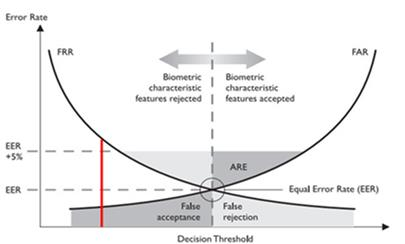
\includegraphics[width=12cm]{Biometrics-Error-Rates.jpg}
\caption{Graficzne przedstawienie FAR, FRR, ERR. (Żródło: ISC2, International Information Systems Security Certification Consortium)}
\end{figure}



  
  Fałszywa akceptacja zachodzi, gdy algorytm klasyfikuje podpis osoby nieuprawnionej za prawdziwy; fałszywe odrzucenie - gdy podpis osoby uprawnionej zostaje zaklasyfikowany jako fałszywy. W praktyce jako parametr porównywania skuteczności różnych metod weryfikacji stosuje się EER - im niższy, tym metoda jest lepsza. \\
  
  Współczynniki te oblicza się następująco:
  \begin{equation*}
      FAR = \frac{liczba falszywie zaakceptowanych}{liczba prob weryfikacji}
  \end{equation*}
  \begin{equation*}
      FRR = \frac{liczba falszywie odrzuconych}{liczba prob weryfikacji}
  \end{equation*}
  
\chapter*{Czego nie udało się zrealizować}
Pośród rzeczy, których nie udało nam się (w całości) zrealizować (z różnych powodów) są:
 \begin{itemize}
  \item funkcjonalność odrzucania podpisów, które wykroczyły poza pole wprowadzania;
  \item funkcjonalność pobierania formularza od IC Solutions i wykrywania pola wprowadzania podpisu;
  \item zbieranie informacji o kątach pisania;
  \item dopracowanie algorytmów weryfikacji i stworzenie algorytmów opartych na innych metodach (np. Ukrytych Modelach Markowa);
  \item wyznaczenie stałego progu dla akcpetacji podpisu (dla każdego autora wyznaczany jest indywidualny próg na podstawie 5 podpisów wzorcowych);
  \item stworzenie statystyk dla różnych algorytmów.
 
 \end{itemize}
 
\chapter*{Wnioski}

\chapter*{Bibliografia}



\end{document}